\documentclass[10pt]{article}
\usepackage{graphicx}
\usepackage{amsmath}

%opening
\title{AI: Answer to Homework 4}
\author{vishvAs vAsuki}

\begin{document}

\maketitle

\section{Question}

  (15\%) Problem 13.9 from R\&N. It is quite often useful to consider the effect of some specific proposition in the context of some general background evidence that remains fixed, rather than the complete absense of information.

   1. Prove the conditionalized version of the general product rule: $P(X,Y|e) = P(X|Y,e)P(Y|e)$.

   2. Prove the conditionalized version of Bayes' rule: 

$P(Y|X,e) = P(X|Y,e) P(Y|e) / P(X|e)$. 

\subsection{Solution}

\paragraph{1} $P(X|Ye)P(Y|e)=\frac{P(X,Y,e)}{P(Ye)}\frac{P(Y,e)}{P(e)} = \frac{P(X,Y,e)}{P(e)}$

But, $P(X,Y|e)=\frac{P(X,Y,e)}{P(e)} $.

Hence, $ P(X|Ye)P(Y|e) = P(X,Y|e)$ QED.


\paragraph{2} As shown above, $P(X|Y,e)P(Y|e) = P(X,Y|e)$.

But, following the same reasoning as above, $P(X,Y|e)=P(Y|X,e)P(X|e)$

Hence, $ P(X|Ye)P(Y|e) = P(Y|X,e)P(X|e)$

So, $P(Y|X,e) = P(X|Y,e) P(Y|e) / P(X|e)$

\section{Question}
 (15\%) Problem 13.15 from R\&N. Suppose you are a witness to a nighttime hit-and-run accident involving a taxi in Athens. All taxis in Athens are blue or green. You swear, under oath, that the taxi was blue. Extensive testing shows that, under the dim lighting conditions, discrimination between blue and green is 75\% reliable. Is it possible to calculate the most likely color of the taxi? (Hint: distinguish between the proposition that the taxi is blue and the proposition that it appears blue.)
What about now, given that 9 out of 10 Athenian taxis are green?

\subsection{Solution}

Let `T=b' indicate the event where the taxi is blue. Also, `T=g' indicates the event where the taxi is green.

Let `A=b' indicate the event where the taxi appears blue. Also, `A=g' indicates the event where the taxi appears green.

We are told that $P(A=b|T=b) = .75$, and $P(A=g|T=g) = .75$. This means that $P(A=b|T=g) = .25$ and $P(A=g|T=b) = .25$.

We are asked to find $P(T=b|A=b)$ and $P(T=g|A=b)$.

\begin{equation}
\begin{split}
P(T=b|A=b)=\frac{P(A=b|T=b)P(T=b)}{P(A=b)}\\
But, P(A=b) = P(A=b,T=b)+P(A=b,T=g)\\
P(A=b) = P(A=b|T=b)P(T=b)+P(A=b|T=g)P(T=g)\\
P(T=b|A=b)=\frac{P(A=b|T=b)P(T=b)}{P(A=b|T=b)P(T=b)+P(A=b|T=g)P(T=g)}\\
\end{split}
\end{equation}

Hence, we can answer the question if we are given $P(A=b|T=b), P(A=b|T=g), P(T=g), P(T=b)$, and not before. We are told that P(T=g)=0.9 and P(T=b)=0.1.

Using the values given, $P(T=b|A=b)=\frac{.75*0.1}{.75*.1+.25*.9}=0.25$

And, $P(T=g|A=b) = 1-P(T=b|A=b)= 0.75$. So, it is more likely that the taxi is green in color.

\section{Question}
 (25\%) Consider the following Bayesian network:

\begin{center}
 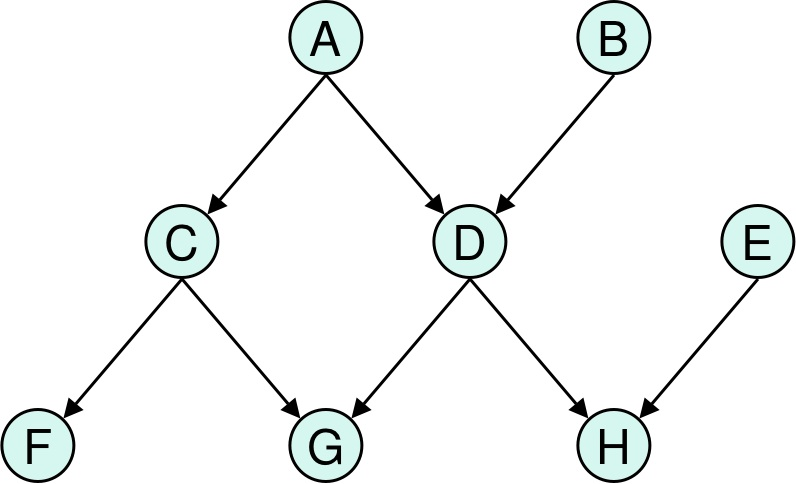
\includegraphics[scale=0.5]{hw4_files/hw4f1.jpg}
 % hw4_files/hw4f1.jpg: 0x0 pixel, 0dpi, nanxnan cm, bb=
\end{center}

   1. Suppose that all the variables are Boolean. How many parameters (real numbers) are needed to specify an arbitrary joint probability distribution over 8 variables? How many parameters are needed to define the joint probability distribution using the above Bayesian network?

   2. Which of the following probabilistic relations are implied by the structure of the above Bayesian network? Explain briefly.

      (a)   	$P(E|G) = P(E)$

      (b)	$P(C|D) = P(C)$

      (c)	$P(C|D,A) = P(C|A)$

      (d)	$P(B|A,C) = P(B|A)$

      (e)	$P(C,D|E) = P(C,D)$

      (f)	$P(F|A,E,H) = P(F|A)$

      (g)	$P(A,C|D,E,H) = P(A,C|D)$

   3. Express $P(A|G)$ in terms of the probabilities directly available in the network. You will need to use Bayes' rule and conditioning on one or more other variables.

\subsection{Solution}

\paragraph{1} $2^{8}-1$ real numbers are required to specify an arbitrary joint probability distribution over 8 variables. For the given Bayesian network, 19 parameters are needed.

\paragraph{2}
      (a)   	$P(E|G) = P(E)$ True. G and E are indeed independent of each other.

      (b)	$P(C|D) = P(C)$ True. C and D are indeed independent of each other.

      (c)	$P(C|D,A) = P(C|A)$ True. C and D are conditionally independent of each other, given A's value.

      (d)	$P(B|A,C) = P(B|A)$ True. B and C are conditionally independent of each other given A.

      (e)	$P(C,D|E) = P(C,D)$ True. The value of E does not affect the outcome of either C or D.

      (f)	$P(F|A,E,H) = P(F|A)$ True. The values of E and H do not affect the value of F, given A's value.

      (g)	$P(A,C|D,E,H) = P(A,C|D)$ True. The values of E and H do not affect the values of A and C, given D's value.

\paragraph{3} 
\begin{equation}
\begin{split}
P(A|G) = \frac{P(G|A)P(A)}{P(G)} 
= \frac{P(A)\Sigma_{C,D,B}P(G|C,D)P(C|A)P(D|A,B)P(B)}{\Sigma_{A,C,D,B} P(G|CD)P(C|A)P(D|A,B)P(A)P(B)}
\end{split}
\end{equation}

\section{Question}
 (20\%) Suppose that in a polytree network, X is an ancestor of Y and we wish to compute $P(Y|X)$ in terms of the CPT entries of the network. Explain why this computation can be done using conditioning operations only and write a general expression for $P(Y|X)$. (Hint: you may find it useful to consider an example such as the following, although the specific details of the example need not appear in your answer.)

\begin{center}
 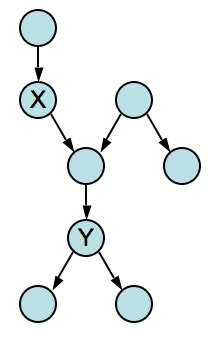
\includegraphics[scale=0.5]{hw4_files/hw4f2.jpg}
 % hw4_files/hw4f1.jpg: 0x0 pixel, 0dpi, nanxnan cm, bb=
\end{center}

\subsection{Solution}

Let the node between X and Y be named B. Let B's unlabelled parent be given the label A.

\begin{equation}
Then, P(Y|X) = \Sigma_{A,B}P(Y|B)P(B|AX)P(A)
\end{equation}

This is because, when we calculate the value of $P(Y|X=x)$, we know the value of X. So, the values of parents of X are irrelevant. Also, according to the given graphical model, the value of P(Y|X) is independent of the children of all the leaf nodes in the graph. So, we need only marginalize over the values of A and B. So, for any x, we can find the value of $P(Y|X=x)$ by only using the conditional probability table of B and the probability table for A.

Hence, $P(Y|X)$ can be calculated using conditional operations only.

\section{Question}
 (25\%) You are an AI consultant for an auto insurance company. Your task is to construct a Bayesian network that will allow the company to decide how much financial risk they run from various policy holders, given certain data about the policy holders. In order to design a Bayesian network, you need output variables and evidence variables. The output variables are those for which the insurance company is trying to get a probability distribution for their possible values. The evidence variables are those variables for which you can obtain information, on the basis of which it is legal to make decisions, and that are relevant to the decision. Output variables represent the cost of various catastrophic events that the insurance company might have to reimburse. In the automobile insurance domain, the major output variables are the medical cost (MedCost), property cost (PropCost), and intangible liability cost (ILiCost). Medical and property costs are those incurred by all individuals involved in an accident; auto theft or vandalism might also incur property cost. Intangible liability costs are legal penalties for things like``pain and suffering,'' punitive damages, and so forth, that a driver might incur in an accident in which he or she is at fault. Evidence variables for this domain include the driver's age and record; whether or not he or she owns another car; how far he or she drives per year; the vehicle's make, model and year; whether it has safety equipment such as airbag and antilock brakes; where it is garaged and whether it has an antitheft device.

   1. Build a possible belief network for this problem. You will need to decide on suitable domains for the variables, bearing in mind the need to discretize. You will also need to add intermediate nodes such as DrivingSkill and AutoRuggedness.

   2. Give reasonable conditional probability tables to a few (but not all!) nodes.

   3. How many independent values are necessary to define the joint probability distribution of your model, assuming no conditional independence relations hold among the variables? How many independent values are needed to complete your model using the conditional independence relations? 

\subsection{Solution}

\paragraph{1} A possible belief network (at least in the universe I imagine) is shown below:

 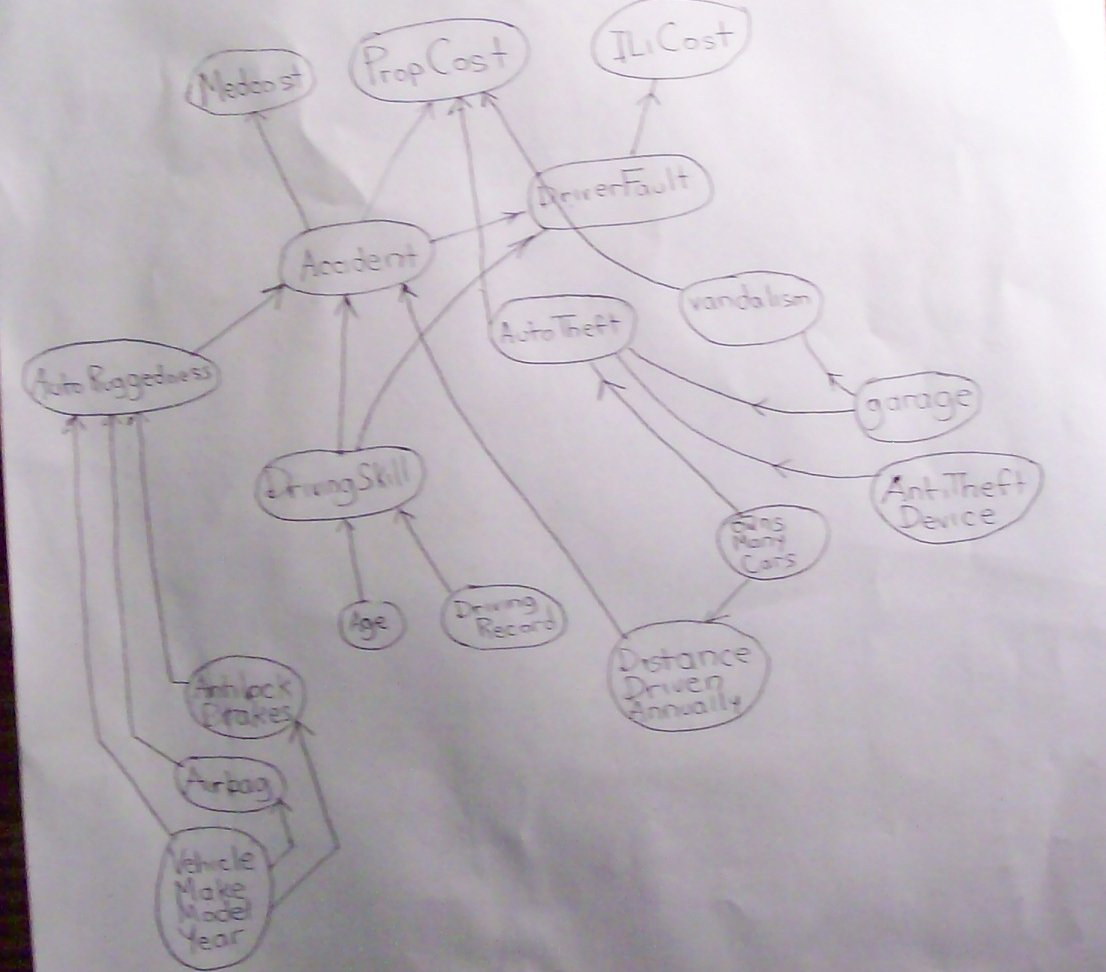
\includegraphics[scale=0.4]{hw4_files/hwBayesNet.jpg}
 % hw4_files/hwBayesNet.jpg: 0x0 pixel, 0dpi, nanxnan cm, bb=

I briefly describe the domains of the variables in the network (Note the domain of `Accident'.):

\begin{itemize}
 \item VehicleMakeModelYear: The set of all Vehicle Make-Model-Year combinations.
 \item Airbag: Boolean.
 \item AntilockBrakes: Boolean.
 \item AutoRuggedness: Integral scale ranging from 1 to n.
 \item Age: suitably defined age intervals.
 \item DrivingRecord: Integral scale ranging from 1 to n.
 \item DrivingSkill: Integral scale ranging from 1 to n.
 \item Accident: Integral scale ranging from 0 to n, encoding the severity of the accident.
 \item DistanceDrivenAnnually: suitably defined distance intervals.
 \item OwnsManyCars: Boolean
 \item AutoTheft: Boolean
 \item AntitheftDevice: Boolean
 \item Garage: Boolean
 \item Vandalism: Boolean
 \item DriverFault: Boolean
 \item MedCost: suitably defined cost intervals.
 \item PropCost: suitably defined cost intervals.
 \item ILICost: suitably defined cost intervals.
\end{itemize}

\paragraph{2} I provide conditional probability tables for the Vandalism, MedCost and ILICost variables.

\begin{tabular}{ll}
 Garage & $P(Vandalism=true|Garage)$ \\
 true & 0.01\\
 false & 0.1\\
\end{tabular} 

Note: $P(Medcost<=\$500|Accident)$ is not shown below.

\begin{tabular}{lll}
 Accident (6 severity levels) & $P(\$500<MedCost<=\$5000|Acc)$ & $P(\$5000<MedCost|Acc)$\\
 0 & 0 & 0\\
 1 & 0.2 & 0.1\\
 2 & 0.2 & 0.2\\
 3 & 0.3 & 0.3\\
 4 & 0.2 & 0.4\\
 5 & 0.1 & 0.4\\
\end{tabular} 

Note: $P(ILIcost<=\$500|Driverfault)$ is not shown below.

\begin{tabular}{lll}
 DriverFault &$P(\$500<ILIcost<=\$5000|Driverfault)$ & $P(\$5000< ILIcost|Driverfault)$\\
 False & 0 & 0\\
 True & 0.2 & 0.3\\
\end{tabular} 

\paragraph*{3}
Let us assume that the variables' domains, described above, are descretized so as to be \textit{binary}. I have defined 18 variables. If there were no conditional independence relationships, then I would need $2^{18}-1$ values to store the joint probability distribution.

But, since I recognize the conditional independence relationships indicated by the network, I only need to store 58 values.

\end{document}
